%% Testable-Auswertung; Datenbasis main b0ac28be3ab0c29d6643f073cb555f087769a8f2.
\section{Explorative Auswertung der Testable-Erhebung}
\label{sec:testable-auswertung}
% Generated by analyse_testable.R; do not edit numbers manually.
\newcommand{\TestableN}{66}
\newcommand{\TestableM}{61,42}
\newcommand{\TestableL}{60,81}
\newcommand{\TestableSDM}{17,52}
\newcommand{\TestableSDL}{16,88}
\newcommand{\TestableDiff}{-0,61}
\newcommand{\TestableSDDiff}{5,24}
\newcommand{\TestableLower}{-1,90}
\newcommand{\TestableUpper}{0,68}
\newcommand{\TestableT}{-0,948}
\newcommand{\TestableP}{0,346}
\newcommand{\TestableDz}{-0,117}
\newcommand{\TestableWilcoxonP}{0,678}
\newcommand{\TestableWilcoxonV}{977,5}
\newcommand{\TestableBootLo}{-1,90}
\newcommand{\TestableBootHi}{0,62}
\newcommand{\TestableAge}{40,95}
\newcommand{\TestableSDAge}{8,52}
\newcommand{\TestableCigs}{13,85}
\newcommand{\TestableSDCigs}{3,78}
\newcommand{\TestableDuration}{117,87}
\newcommand{\TestableDurationQone}{114,61}
\newcommand{\TestableDurationQthree}{132,38}


\subsection{Datenbasis und technische Rekonstruktion}
Die browserbasierte Testable-Erhebung wird als eigenständige Umsetzung des Vergleichs zwischen Cue-Matching und Cue-Labeling ausgewertet. Sie unterscheidet sich hinsichtlich Zeitplan, Endgeräten und Aufgabenpräsentation von der mehrtägigen App-Studie. Ihre Daten werden deshalb nicht mit den App-Selbstberichten zusammengeführt. Grundlage sind das versionierte \path{cuelens_testable.org/trial_file.csv} und die 68 Ergebnisdateien des Exportverzeichnisses \path{996939_20260916_153409_all} im Repository-Stand \texttt{b0ac28b} vom 20. September 2026.\footnote{Vollständiger Commit: \url{https://github.com/stefan-bmio/master-thesis/tree/b0ac28be3ab0c29d6643f073cb555f087769a8f2}. Die Dateiprüfsummen sind im Auswertungspaket dokumentiert.}

Die CSV-Exporte bestehen aus zwei Tabellen: einem Metadatenkopf und der eigentlichen Ergebnistabelle. Beide Teile werden getrennt eingelesen.\footnote{Zur Exportstruktur siehe Testable, \emph{How to Read the Results Files}: \url{https://www.testable.org/docs/feature-manual/how-to-read-results/}, abgerufen am 21. September 2026.} Die Auswertung verwendet Teilnehmerkennung, Trial-Version, Antworten, Trial-Zeilennummern und Zeitangaben. Freitextantworten und individuelle Kennungen werden nicht in die veröffentlichten Ergebnistabellen übernommen. Die exportierten Betriebssystemangaben beschreiben die Browserumgebung; sie werden nicht als sicherer Nachweis eines bestimmten Gerätetyps interpretiert.

Das Trial-File enthält 20 Blöcke mit je fünf Bildaufgaben und anschließendem Craving-Selbstbericht. Ungerade Blöcke verwenden Matching, gerade Blöcke Labeling. Damit sind 50 Aufgaben je Bedingung und zehn Selbstberichte je Bedingung vorgesehen. Der Slider reicht von 0 bis 100 in Einerschritten und ist auf 50 voreingestellt. Zwischen den Blöcken sind 19 Pausen mit einem Fünf-Minuten-Timer konfiguriert. Vor jeder Matching-Antwort steht zusätzlich eine \texttt{learn}-Zeile mit einem Fünf-Sekunden-Timer; bei Labeling fehlt diese zusätzliche Präsentation. Die Antwortpositionen sind im vorliegenden Trial-File festgelegt; eine Gegenbalancierung der Reihenfolge Matching--Labeling ist darin nicht enthalten.

Die 100 Bildentscheidungen sind als \texttt{practice} angelegt und fehlen in den vorliegenden Ergebnisexporten. Auch die Pausenfrage nach Block 5 ist als \texttt{practice} konfiguriert. Pro Datei liegen deshalb 40 exportierte Ergebniszeilen vor: zwei Screening-Antworten, 20 Slider-Einträge und 18 Pausenfragen. Aus diesen Exporten lassen sich weder Richtigkeit noch Reaktionszeiten der Bildentscheidungen prüfen. Die vollständigen Craving-Daten sind somit kein Nachweis korrekter Bearbeitung aller Zuordnungsaufgaben.

Die Zuordnung der Selbstberichte zu den Bedingungen erfolgt über \texttt{rowNo} und die aus dem Trial-File rekonstruierte Blockstruktur. Die erwarteten Zeilennummern lauten
\begin{quote}\small
16, 25, 39, 48, 62, 71, 85, 94, 108, 117, 131, 140, 154, 163, 177, 186, 200, 209, 223, 232.
\end{quote}
Eine bloß abwechselnde Kennzeichnung exportierter Antworten wäre fehleranfällig: Zusätzliche oder fehlende Einträge würden alle folgenden Bedingungszuordnungen verschieben. Die Pipeline prüft daher explizit Zeilenzuordnung, Eindeutigkeit, Wertebereich und zeitliche Reihenfolge. Die in diesen Dateien gespeicherten \texttt{timestamp}-Werte werden als Millisekunden seit Sitzungsbeginn interpretiert; ihre Größenordnung und der letzte Wert passen zur Metadatenvariable \texttt{duration\_s}.

Die Zuordnung setzt voraus, dass das vorliegende Trial-File den Ablauf der exportierten Erhebung hinsichtlich der Blockbedingungen korrekt abbildet. Die Zeilennummern und Frageinhalte der Selbstberichte sind damit vereinbar. Eine vollständige Identitätsprüfung der nicht exportierten Bildaufgaben gegenüber der in Testable eingesetzten Upload-Version ist anhand dieser Dateien jedoch nicht möglich. Der Git-Stand dokumentiert den gesicherten Analyseinput, nicht automatisch die vollständige Plattformkonfiguration zum Erhebungszeitpunkt.

\subsection{Analysestichprobe und Datenqualität}
Von den 68 Dateien tragen 67 eine eindeutige Teilnehmerkennung und die exportierte Trial-Version \texttt{2026-09-15\_17:52:16}. Eine weitere Sitzung vom 14. September besitzt keine Teilnehmerkennung und stammt aus der Version \texttt{2026-09-14\_15:28:43}. Ihre Herkunft als reguläre Teilnahme oder technischer Probelauf ist aus dem Export allein nicht abschließend bestimmbar. Sie wird aus der Hauptanalyse ausgeschlossen und in einer Sensitivitätsanalyse zusätzlich berücksichtigt.

Eine identifizierte Sitzung enthält neben Zeile 16 den zusätzlichen Eintrag \texttt{16\_2}, jedoch keinen Bericht für Zeile 232. Die beiden Einträge zum ersten Bericht enthalten denselben Craving-Wert. Somit entsprechen 20 exportierte Slider-Einträge in diesem Fall nur 19 verschiedenen vorgesehenen Messzeitpunkten. Diese Sitzung geht nicht in die vollständige Hauptanalyse ein. In einer ergänzenden Auswertung werden ihre neun vollständigen Matching--Labeling-Blockpaare verwendet; der zusätzliche Eintrag wird nicht als unabhängige Messung gewertet und der letzte Bericht nicht imputiert.

Die Hauptanalyse umfasst damit \TestableN{} Personen mit jeweils 20 eindeutig zugeordneten und gültigen Berichten, insgesamt 1320 Messwerten. Alle erfüllen die im Trial-File implementierten Screening-Grenzen von mindestens 30 Jahren und mindestens zehn Zigaretten pro Tag. Eine obere Altersgrenze wird im Trial-File nicht geprüft. Da Kapitel 6 für die App-Studie höchstens 65 Jahre vorsieht, wird zusätzlich eine Analyse ohne die eine 67-jährige Person berichtet. Die übrigen für die App beschriebenen Kriterien, insbesondere Wohnsitz und App-Nutzung, können aus diesen Exporten nicht vollständig nachgeprüft werden.

Das mittlere Alter beträgt \TestableAge{} Jahre (SD \TestableSDAge{}; Spannweite 30--67), die angegebene tägliche Zigarettenzahl im Mittel \TestableCigs{} (SD \TestableSDCigs{}; Spannweite 10--25). Die Sitzungsdauer liegt im Median bei \TestableDuration{} Minuten (Interquartilsbereich \TestableDurationQone{}--\TestableDurationQthree{} Minuten). Als Betriebssystem sind Windows für 42, Android für neun, MacOS und UNIX für jeweils sechs sowie iOS für drei Personen angegeben. Die Daten stammen somit nicht ausschließlich aus einer Smartphone-Umgebung.

Bei fünf vollständigen Teilnahmen sind zusammen 49 der insgesamt 1254 Abstände zwischen aufeinanderfolgenden Selbstberichten kürzer als 300 Sekunden. Da in diesen Abstand zusätzlich zu einer Pause auch Aufgabenbearbeitung und Antwortzeit fallen, ist ein solcher Abstand mit einer vollständig eingehaltenen Fünf-Minuten-Pause unvereinbar, sofern die Zeitstempel korrekt sind. Umgekehrt beweist ein längerer Abstand allein nicht die Einhaltung der Pause. Die betroffenen Teilnahmen bleiben in der Hauptanalyse erhalten; die ergänzende Analyse ohne sie prüft die Robustheit gegenüber dieser Auffälligkeit. Eine Person mit konstanten Craving-Angaben wird ebenfalls beibehalten: Konstanz allein belegt keine ungültige Teilnahme. Es werden keine Personen aufgrund der Richtung oder Größe ihres Bedingungsunterschieds ausgeschlossen.

Die Dateizahl erlaubt keine Bestimmung der Rekrutierungs-, Abbruch- oder Abschlussquote, weil Angaben zur Gesamtheit der begonnenen Teilnahmen und ausgeschlossenen Personen fehlen. Ebenso beweisen die Exporte allein keine dokumentierte Einwilligung oder Einhaltung der Bitte, während der Erhebung nicht zu rauchen.

\subsection{Statistisches Vorgehen}
Die Berechnungen wurden mit R 4.3.3 und den mitgelieferten Paketen durchgeführt.\footnote{R Core Team (2024), \emph{R: A Language and Environment for Statistical Computing}, R Foundation for Statistical Computing, Wien; \url{https://www.R-project.org/}. Funktionsdokumentation: \url{https://stat.ethz.ch/R-manual/R-patched/library/stats/html/t.test.html}.} Die vorliegende Testable-Auswertung wurde nach der Datenerhebung festgelegt und ist explorativ; eine Präregistrierung dieses Analyseplans liegt ihr nicht zugrunde. Die im Arbeitsprotokoll festgehaltenen Auswahlregeln wurden nach der strukturellen Datenprüfung und vor Berechnung der inferenzstatistischen Ergebnisse definiert. Abweichend von der einseitigen Fallzahlplanung der App-Studie werden hier zweiseitige Tests und 95\,\%-Konfidenzintervalle berichtet.

Für jede Person $i$ werden zunächst die zehn Matching- und zehn Labeling-Werte gemittelt. Der zentrale Kontrast ist
\begin{equation}
 D_i=\overline{Y}_{i,L}-\overline{Y}_{i,M},\qquad
 \widehat{\Delta}=\frac{1}{n}\sum_{i=1}^{n}D_i.
\end{equation}
Negative Werte bedeuten geringeres Rauchverlangen nach Labeling. Jede Person erhält dasselbe Gewicht. Die 1320 Einzelberichte werden nicht als unabhängige Beobachtungen behandelt. Der Ein-Stichproben-$t$-Test der Personendifferenzen gegen null ist rechnerisch identisch mit einem gepaarten $t$-Test der beiden Personenmittelwerte. Berichtet werden außerdem die Standardabweichung $s_D$, das Intervall
\begin{equation}
 \widehat{\Delta}\ \pm\ t_{n-1;0{,}975}\frac{s_D}{\sqrt{n}}
 \quad\text{und}\quad d_z=\frac{\widehat{\Delta}}{s_D}.
\end{equation}
Die Inferenz setzt unabhängige Personen und eine hinreichend geeignete Stichprobenverteilung des Mittelwerts der Differenzen voraus. Als Robustheitsprüfungen dienen ein Wilcoxon-Vorzeichenrangtest mit Normalapproximation und Kontinuitätskorrektur sowie ein Perzentil-Bootstrap mit 10000 Ziehungen auf Personenebene und festem Zufallsstartwert. Der Wilcoxon-Test prüft eine Lagehypothese unter einer Symmetrieannahme und ist daher kein identischer Test derselben Mittelwertshypothese.

Zusätzliche Sensitivitätsanalysen beziehen die ältere Sitzung ein, nutzen die verfügbaren vollständigen Blockpaare der unvollständigen Teilnahme oder beschränken Alter bzw. Berichtsabstände. Zur Untersuchung des Zeitverlaufs werden außerdem je Person lineare Modelle
\begin{equation}
 Y_{ib}=\alpha_i+\beta_i I(L_b)+\gamma_i t_{ib}+\varepsilon_{ib}
\end{equation}
geschätzt. Dabei ist $t_{ib}$ alternativ die Blocknummer oder die tatsächlich seit dem ersten Selbstbericht verstrichene Zeit. Anschließend werden die personenspezifischen Bedingungskoeffizienten $\beta_i$ gemittelt und mit einem $t$-Intervall über Personen zusammengefasst. Diese Modelle erlauben unterschiedliche lineare Zeittrends je Person; sie beseitigen jedoch keine beliebigen nichtlinearen Verläufe, Übertragungseffekte oder systematischen Präsentationsunterschiede. Alle ergänzenden Analysen sind explorativ; ihre $p$-Werte werden ohne Korrektur für multiples Testen ausgewiesen und nicht als zusätzliche konfirmatorische Tests interpretiert.

\subsection{Ergebnisse}
Die personenbezogenen Mittelwerte des Rauchverlangens betragen nach Matching \TestableM{} Punkte (SD \TestableSDM{}) und nach Labeling \TestableL{} Punkte (SD \TestableSDL{}). Die mittlere Differenz Labeling minus Matching ist \TestableDiff{} Punkte (SD der Differenzen \TestableSDDiff{}; 95\,\%-KI [\TestableLower{}; \TestableUpper{}]). Der gepaarte Vergleich ergibt $t(65)=\TestableT$, $p=\TestableP$ und $d_z=\TestableDz$. Damit liefern die Daten keinen statistisch belastbaren Nachweis eines mittleren Unterschieds zwischen den Bedingungen in diesem Ablauf.

Bei 32 Personen ist der Mittelwert nach Labeling niedriger, bei 32 höher; bei zwei Personen sind beide Mittelwerte gleich. Der Median der Personendifferenzen beträgt null. Abbildung~\ref{fig:testable-paired} zeigt sowohl die individuellen Mittelwerte als auch die Streuung ihrer Differenzen.
\begin{figure}[htbp]
 \centering
 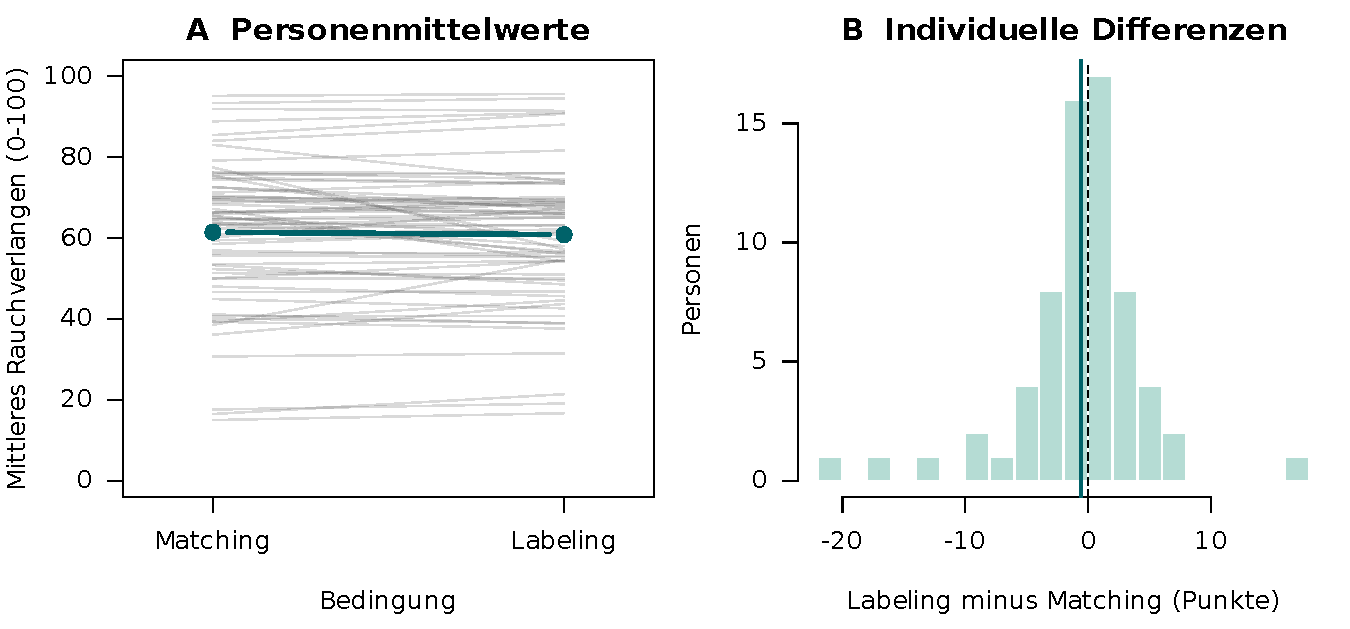
\includegraphics[width=\linewidth]{../analysis/testable/output/testable_results.pdf}
 \caption{Craving nach Matching und Labeling bei 66 vollständigen Teilnahmen. Links verbinden graue Linien die beiden Mittelwerte derselben Person; die hervorgehobene Linie zeigt die Gruppenmittelwerte. Rechts ist die Verteilung der Personendifferenzen dargestellt; gestrichelt ist null, farbig der Mittelwert markiert.}
 \label{fig:testable-paired}
\end{figure}

Der Wilcoxon-Test ergibt $V=\TestableWilcoxonV$ und $p=\TestableWilcoxonP$. Das Bootstrap-Intervall reicht von \TestableBootLo{} bis \TestableBootHi{} Punkten. Beide Robustheitsprüfungen stützen die vorsichtige Interpretation der Hauptanalyse. Die weiteren Varianten sind in Tabelle~\ref{tab:testable-sensitivity} vollständig aufgeführt; keine liefert bei einem zweiseitigen Niveau von 5\,\% einen statistisch signifikanten Bedingungsunterschied.
\begin{table}[htbp]
 \centering\small
 \setlength{\tabcolsep}{3pt}
 \begin{tabular}{p{.38\linewidth}rrrr}
\toprule
Analyse & $n$ & Differenz & 95\,\%-KI & $p$ \\
\midrule
Hauptanalyse & 66 & -0,61 & [-1,90; 0,68] & 0,346 \\
Mit älterer Sitzung ohne Kennung & 67 & -0,72 & [-2,00; 0,57] & 0,269 \\
Verfügbare Blockpaare & 67 & -0,61 & [-1,88; 0,66] & 0,344 \\
Altersgrenze 65 Jahre & 65 & -0,62 & [-1,93; 0,69] & 0,347 \\
Alle Berichtsabstände mindestens 5 min & 61 & -0,78 & [-2,12; 0,57] & 0,252 \\
Linearer Blocktrend je Person & 66 & -0,92 & [-2,19; 0,34] & 0,149 \\
Linearer Zeittrend je Person & 66 & -0,91 & [-2,17; 0,35] & 0,154 \\
\bottomrule
\end{tabular}

 \caption{Explorative Sensitivitätsanalysen. Differenzen und Konfidenzintervalle in Punkten der Skala 0--100. Negative Werte entsprechen geringerem Rauchverlangen nach Labeling. Bei den beiden Trendmodellen wird der mittlere personenspezifische Bedingungskoeffizient berichtet.}
 \label{tab:testable-sensitivity}
\end{table}

Abbildung~\ref{fig:testable-course} stellt die Gruppenmittelwerte nach Block dar. Die Fehlerbalken sind punktweise Konfidenzintervalle für den jeweiligen Blockmittelwert; aus ihrer Überlappung lässt sich kein gepaarter Bedingungstest ableiten. Der letzte Selbstbericht liegt im Mittel 6,11 Punkte über dem ersten (95\,\%-KI [$-3{,}16$; $15{,}37$]). Dieser Anfang-Ende-Vergleich vermischt Zeitverlauf und Bedingung, da die Erhebung mit Matching beginnt und mit Labeling endet; er wird ausschließlich deskriptiv interpretiert.
\begin{figure}[htbp]
 \centering
 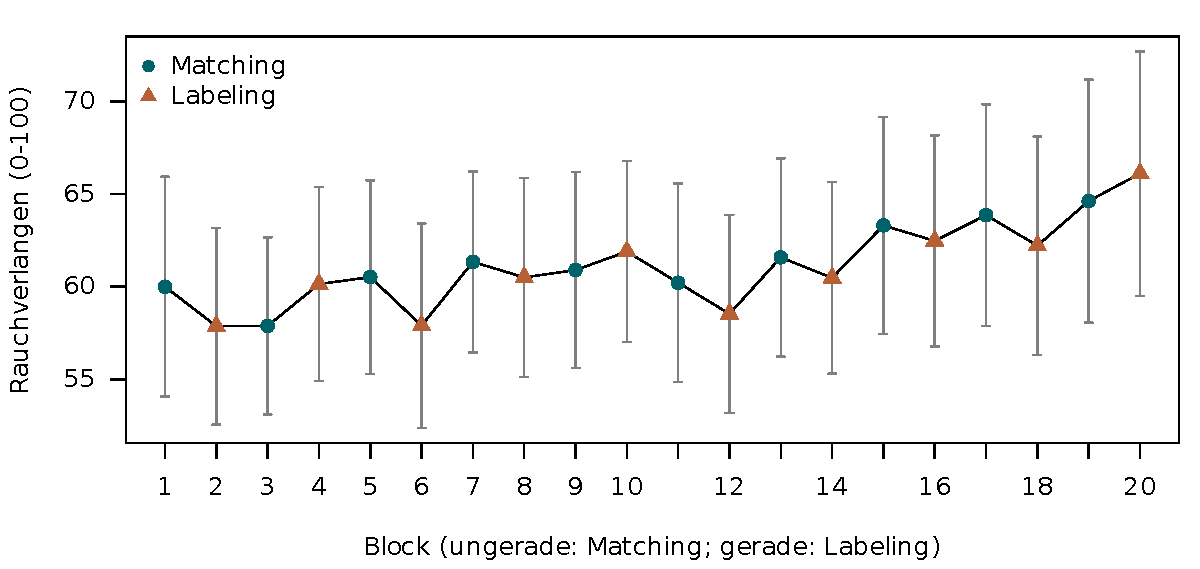
\includegraphics[width=\linewidth]{../analysis/testable/output/testable_timecourse.pdf}
 \caption{Verlauf des mittleren Rauchverlangens über die 20 Blöcke bei denselben 66 Personen. Fehlerbalken: punktweise 95\,\%-Konfidenzintervalle über Personen. Die Bedingungen wechseln in fester Reihenfolge.}
 \label{fig:testable-course}
\end{figure}

\subsection{Wissenschaftliche Einordnung und Konsequenzen}
Die Punktschätzung liegt zwar in der erwarteten Richtung eines geringeren Rauchverlangens nach Labeling, ist jedoch klein und mit null sowie mit geringfügig höherem Rauchverlangen vereinbar. Ein nicht signifikanter Test beweist weder Gleichwertigkeit noch Wirkungslosigkeit. Eine klinisch relevante Veränderung wurde für diese konkrete Operationalisierung nicht vorab definiert; zudem fehlen ein unbehandelter Vergleich, eine Messung vor jedem Aufgabenblock und ein Endpunkt zum Rauchstopp. Die Ergebnisse dürfen deshalb nicht als Beleg einer therapeutischen Wirksamkeit oder deren genereller Abwesenheit formuliert werden.

Die feste Reihenfolge ist die zentrale Grenze der kausalen Interpretation. Jede Labeling-Messung liegt später als die vorangehende Matching-Messung. Zeit seit der letzten Zigarette, Gewöhnung, Ermüdung, Tätigkeiten während der Pausen und Übertragungseffekte können deshalb mit dem Bedingungskontrast zusammenhängen. Hinzu kommen die unterschiedlichen Präsentationsabläufe und die fehlenden exportierten Bildantworten. Die linearen Sensitivitätsmodelle beschränken lediglich eine bestimmte Form des Zeittrends; sie ersetzen keine randomisierte oder gegenbalancierte Zuweisung. Auch ein statistisch signifikanter Unterschied wäre unter diesen Voraussetzungen nicht eindeutig dem Cue-Labeling zuzuschreiben.

Für die medizinisch-informatische Bewertung zeigt die Auswertung zweierlei: Die Rekonstruktion der Messbedingungen und die reproduzierbare Analyse sind mit einem schlanken, versionierten Verfahren möglich. Gleichzeitig ist die technische Verfügbarkeit von CSV-Dateien nicht mit vollständiger experimenteller Nachvollziehbarkeit gleichzusetzen. Zukünftige Trial-Versionen sollten explizite Block- und Bedingungskennungen exportieren, Bildentscheidungen als auswertbare Trials erfassen, Präsentationszeiten zwischen den Bedingungen angleichen und Reihenfolge sowie Pausenmechanismus vor der Erhebung prüfen. Die Vergleichbarkeit mit der App-Studie erfordert außerdem eine explizite Festlegung von Altersgrenzen, Rekrutierung, Endgeräten und Zeitplan. Diese Änderungen betreffen künftige Erhebungen; sie werden nicht rückwirkend in die vorliegenden Rohdaten eingearbeitet.

\subsection{Reproduzierbarer R-Quelltext}
\label{sec:testable-r-code}
Listing~\ref{lst:testable-r} enthält den vollständigen ausführbaren Quelltext. Er wird aus dem Repository-Hauptverzeichnis mit \texttt{Rscript analysis/testable/analyse\_testable.R} gestartet. Die Funktion \texttt{cairo\_pdf} benötigt eine R-Installation mit Cairo-Unterstützung. Das Skript erzeugt aggregierte CSV-Ergebnisse, zwei Vektorabbildungen, die direkt eingebundenen LaTeX-Zahlen und die Sensitivitätstabelle, ein Prüfsummenverzeichnis sowie \texttt{sessionInfo()}. Dadurch stammen Berechnung, Tabellen und Abbildungen aus derselben Verarbeitung. Die Rohdaten bleiben unverändert. MD5-Prüfsummen dienen hier ausschließlich der Identifizierung des verwendeten Dateistands, nicht als kryptografischer Sicherheitsnachweis.

\lstinputlisting[language=R,basicstyle=\ttfamily\scriptsize,
 numbers=left,numberstyle=\tiny,numbersep=6pt,stepnumber=1,
 breaklines=true,breakatwhitespace=false,columns=fullflexible,
 keepspaces=true,showstringspaces=false,frame=single,
 caption={Vollständige R-Auswertung der Testable-Exporte},label={lst:testable-r}]
 {../analysis/testable/analyse_testable.R}
